
今天所有的高性能计算机都有多个CPU或多个CPU内核(单个包中的独立处理器)。甚至大多数笔记本电脑都至少有两个内核,通常是四个。正如我们已经说过的,在性能的上下文中,高效不会让任何硬件处于空闲。如果程序只使用一小部分计算能力,例如:多个CPU内核中的一个,那么其就不是高效或高性能的。一个程序在同一时间使用多个处理器的方法只有一种:必须运行多个线程或进程。另外,这并不是使用多处理器的唯一方法,例如:很少有笔记本电脑用于高性能计算。相反,它们可以使用多个CPU来更好地同时运行不同且独立的程序。这是一个非常好的模型,只是在高性能计算上下文中不是我们感兴趣的那种。HPC系统通常会在每台计算机上运行程序,甚至在分布式计算的情况下在多台计算机上运行同一个程序。那么程序如何使用多个CPU?通常,可以让程序运行多个线程。

\subsubsubsection{5.2.1\hspace{0.2cm}线程是什么?}

线程是一个指令序列,可以独立于其他线程执行。多个线程可以在同一个程序中并发运行。所有线程共享相同的内存,根据定义,相同进程的线程运行在同一台机器上(HPC程序也可以包含多个进程)。分布式程序可以运行在多台机器上,并可以使用许多进程。分布式计算的主题超出了本书的范围:我们正在了解如何最大化这些进程的性能。

那么,我们能对多线程的性能聊些什么呢?首先,只有当系统有足够的资源能够同时执行多个指令序列时,同时执行多个指令序列才有益。否则,操作系统需要在不同的线程之间切换,以确保每个线程都有时间片可以执行。

单个处理器上,忙于计算的线程提供处理器能够处理的尽可能多的工作,即使线程没有使用所有的计算单元或正在等待内存访问:处理器一次只能执行一个指令序列-它有一个程序计数器。现在,如果线程正在等待某些东西,比如用户输入或网络信息,那么CPU处于空闲状态,可以执行另一个线程,而不会影响第一个线程的性能。这里,操作系统会处理线程之间的切换。注意,等待内存并不算等待:当一个线程等待内存时,只是需要更长的时间来执行一条指令。当一个线程在等待I/O时,必须进行一个操作系统调用,然后该线程会被操作系统阻塞,直到操作系统唤醒它来处理数据,才执行其他操作。

如果目标是提高程序的整体效率,那么执行繁重计算的线程就需要有足够的资源支持。通常,考虑线程的资源时,我们立即想到的是使用多个处理器或处理器核心。还有其他方法可以通过并发性来提高资源利用率,我们将看到这一点。

\subsubsubsection{5.2.2\hspace{0.2cm}对称多线程}

处理器有很多计算硬件,大多数程序很少可以使用所有的硬件:程序中的数据依赖关系限制了处理器的计算能力。如果处理器有空闲的计算单元,就不能同时执行另一个线程来提高效率吗?这就是对\textbf{称多线程(SMT)}背后的思想,也被称为\textbf{超线程}。

支持SMT的处理器只有一组寄存器和计算单元,但是有两个(或更多)程序计数器和一个计数器副本,用来维护正在运行的线程的状态(具体的实现因处理器的不同而不同)。最终结果是:操作系统将单个处理器视为两个(通常)或多个独立处理器,每个处理器能够运行一个线程。实际上,运行在一个CPU上的线程会竞争共享的资源,比如寄存器。如果每个线程没有充分利用这些共享资源,SMT可以提供显著的性能提高。换句话说,其通过运行多个这样的线程来弥补一个线程的低效。

实际中,大多数支持SMT的处理器都可以运行两个线程,而且性能的提高很大。很少看到100\%的加速(两个线程都以全速运行),通常实际的加速在25\%到50\%之间(第二个线程实际上以四分之一到一半的速度运行),但是有些程序没有加速。出于本书的目的,我们不会以任何特殊的方式对待SMT线程:对于程序来说,SMT处理器就像两个处理器,在不同内核上运行的两个线程性能情况,同样适用于恰好在同一内核上运行的两个线程的性能。这时,必须衡量运行的线程数是否大于物理内核数,并且是否能够为程序提供加速,从而确定要运行多少个线程。

无论是共享整个物理核,还是SMT硬件创建的逻辑核,并发程序的性能在很大程度上取决于工作线程的独立性。这是由算法和线程之间的工作划分决定的,关于这两个问题的书都有数百本之多,但这个问题不在本书的讨论范围内。相反,我们现在关注的是影响线程交互,并决定特定实现成功或失败的因素。

\subsubsubsection{5.2.3\hspace{0.2cm}线程和内存}

由于多个计算线程之间对CPU进行时间切片不会带来性能上的好处,所以在本章的其余部分,可以假设我们在每个处理器核心上运行一个HPC线程(或者在由SMT处理器提供的每个逻辑核心上运行一个线程)。只要这些线程不竞争任何资源,就可以彼此独立地运行,我们就可以享受到加速:两个线程在同一时间内完成的工作是一个线程的两倍。如果工作可以在两个线程之间,以一种独立的方式完美地分配,那么两个线程将在一半的时间内解决问题。

这种理想的情况确实发生过,但并不常见。如果发生这种情况,需要准备好从程序中获得最佳性能,因为我们已经知道了如何优化单个线程的性能。

当不同线程所做的工作不完全独立,并且这些线程开始竞争资源时,编写高效的并发程序就困难了。如果每个线程都充分利用了CPU,那么还有什么其他的东西可以竞争呢?那就是内存了。所有线程都共享内存,因此内存是公共资源。这就是为什么对多线程程序性能的任何探索,几乎都会关注线程之间通过内存交互所产生的问题。

编写高性能并发程序还有另一个方面的能力,就是如何为线程和进程划分工作。但要了解这些,必须找一本关于并行编程的书,里面应该都会有介绍。

事实证明,内存已经是性能的最大瓶颈,添加并发性时,这个问题会放大。硬件所施加的基本限制无法解决问题,大多数程序的性能甚至还没有达到触发这些限制的条件。对于资深的开发者来说,这里有很大的空间来提高代码的效率。即本章为读者提供的知识和工具。

我们首先检查存在线程时内存系统的性能。用上一章的方法,通过测量读或写进内存的速度,只是现在用几个线程同时进行读或写。我们从这样一种情况开始:每个线程都有自己的内存区域可以访问。不是在线程之间共享任何数据,而是共享硬件资源,比如内存带宽。

内存基准测试与我们前面使用的几乎相同,基准函数体是完全相同的,例如:为了对顺序读取进行基准测试,我们使用以下函数:

\hspace*{\fill} \\ %插入空行
\noindent
\textbf{01c\_cache\_sequential\_read.C}
\begin{lstlisting}[style=styleCXX]
template <class Word>
void BM_read_seq(benchmark::State& state) {
	const size_t size = state.range(0);
	void* memory = ::malloc(size);
	void* const end = static_cast<char*>(memory) + size;
	volatile Word* const p0 = static_cast<Word*>(memory);
	Word* const p1 = static_cast<Word*>(end);
	for (auto _ : state) {
		for (volatile Word* p = p0; p != p1; ) {
			REPEAT(benchmark::DoNotOptimize(*p++);)
		}
		benchmark::ClobberMemory();
	}
	::free(memory);
	state.SetBytesProcessed(size*state.iterations());
	state.SetItemsProcessed((p1 - p0)*state.iterations());
}
\end{lstlisting}

注意,内存在基准函数中分配。这个函数需要多个线程调用,每个线程都要有自己读取数据的内存区域,这正是谷歌基准库在运行多线程基准时所做的。要在多个线程上运行基准测试,只需要使用正确的参数即可:

\begin{lstlisting}[style=styleCXX]
#define ARGS ->RangeMultiplier(2)->Range(1<<10, 1<<30) \
			->Threads(1)->Threads(2)
BENCHMARK_TEMPLATE1(BM_read_seq, unsigned long) ARGS;
\end{lstlisting}

可以为不同的线程数指定任意数量的运行,或者使用\texttt{ThreadRange()}参数来生成一个范围为1、2、4、8、…个线程。这里,必须决定要使用多少线程,因为对于HPC基准测试,通常没有理由检查设备拥有的CPU数量(包括SMT)。其他内存访问模式(如随机访问)的基准测试也以同样的方式进行(上一章中的代码)。为了写入,任何值都可以:

\hspace*{\fill} \\ %插入空行
\noindent
\textbf{01d\_cache\_sequential\_write.C}
\begin{lstlisting}[style=styleCXX]
Word fill; ::memset(&fill, 0xab, sizeof(fill));
for (auto _ : state) {
	for (volatile Word* p = p0; p != p1; ) {
		REPEAT(benchmark::DoNotOptimize(*p++ =
		  fill);)
	}
	benchmark::ClobberMemory();
}
\end{lstlisting}

现在展示结果,例如:下面是顺序写的内存吞吐量:

%\hspace*{\fill} \\ %插入空行
\begin{center}
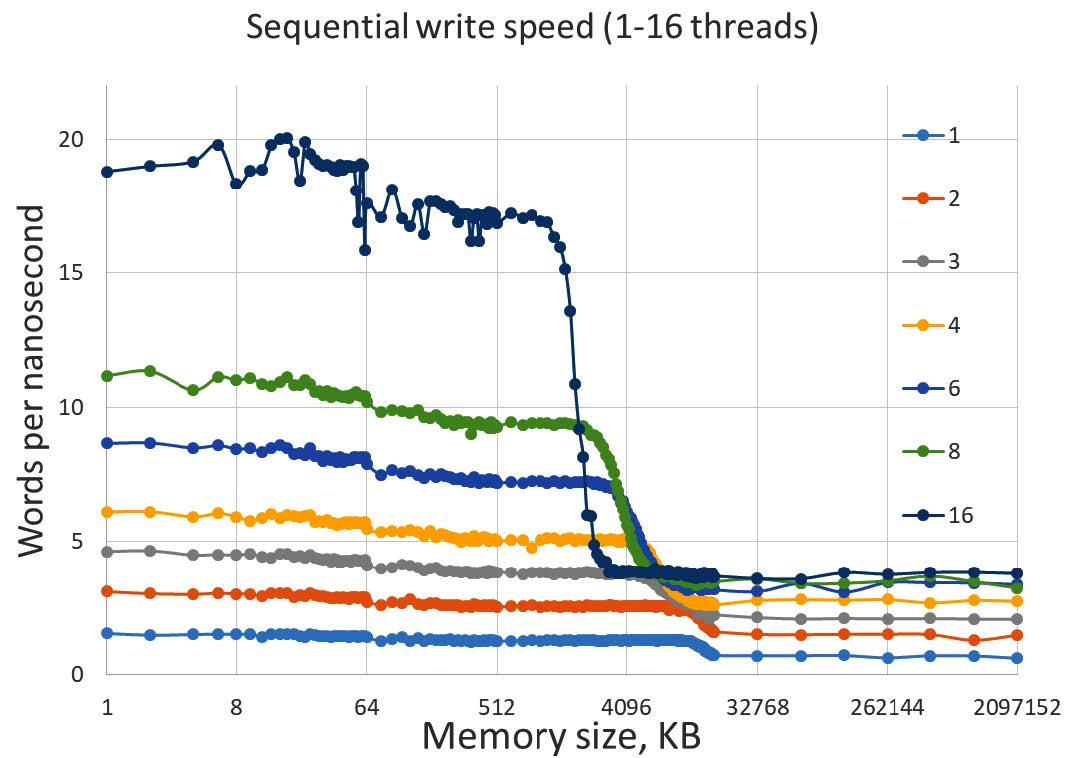
\includegraphics[width=0.9\textwidth]{content/1/chapter5/images/1.jpg}\\
图5.1 - 连续写入64位整数的内存吞吐量(每纳秒字数),线程数的范围为1到16
\end{center}

总的趋势我们已经很熟悉了:我们看到了与缓存大小相对应的速度。现在我们关注不同数量线程的曲线之间的差异,得到了从1到16个线程的结果(用于收集这些测量的机器确实至少有16个物理CPU核)。我们从图的左边开始。这里,速度受到L1缓存(最多32KB)和L2缓存(256KB)的限制。这个处理器对每个核心都有单独的L1和L2缓存,所以只要数据适合L2缓存,线程之间就不应该有交互,因为它们不共享任何资源:每个线程都有自己的缓存。实际上,这并不完全正确,即使在较小的内存范围内,也有CPU组件是共享的。不过,这个结论几乎是正确的:2个线程的吞吐量是1个线程的两倍,4个线程写入内存的速度又快了一倍,16个线程几乎比4个线程快4倍。

当数据超过L2缓存的大小,进入L3缓存,然后进入主存时,情况发生了巨大的变化:这个系统中,L3缓存是在所有CPU内核之间共享的。主内存也是共享的,尽管不同的内存体更接近于不同的CPU(非统一的内存架构)。对于1、2甚至4个线程,吞吐量继续随着线程数量的增加而增加:主内存似乎有足够的带宽,可以支持最多4个处理器的全速写入。然后情况变得更糟:当线程数从6增加到16时,吞吐量几乎没有增加。内存总线已经饱和了,不能更快地写数据了。

如果这还不够糟糕,请考虑这些结果是在撰写本文时(2020年)在最新的硬件上获得的。在2018年时,作者在他的课上展示的图表:

%\hspace*{\fill} \\ %插入空行
\begin{center}
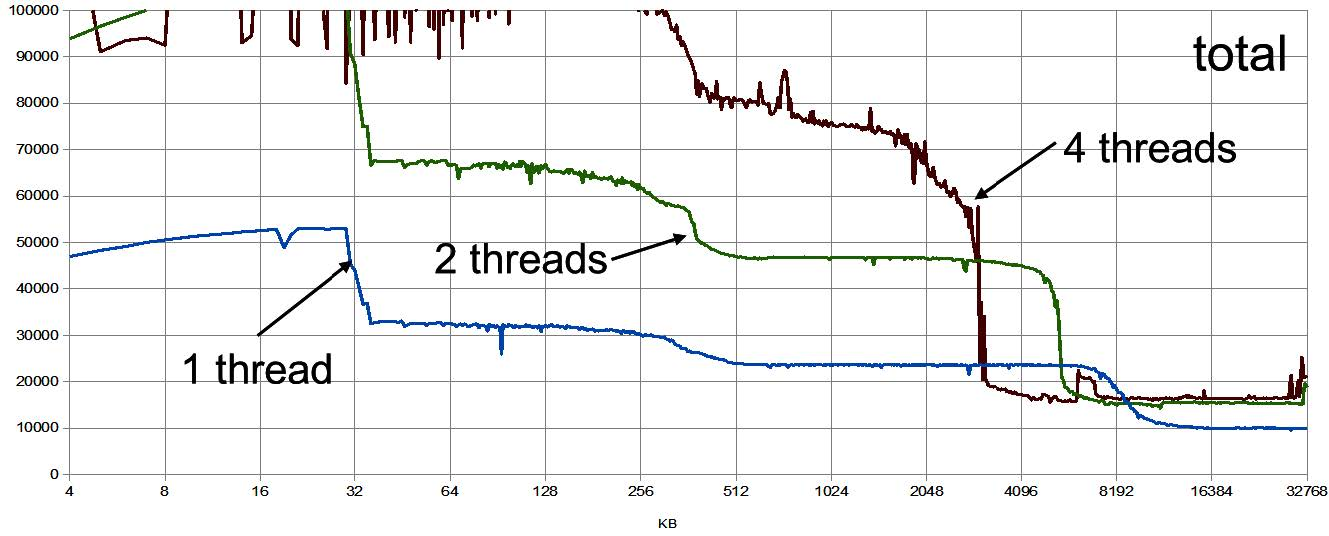
\includegraphics[width=0.8\textwidth]{content/1/chapter5/images/2.jpg}\\
图5.2 -旧CPU(2018)的内存吞吐量
\end{center}

这个系统有一个内存总线,两个线程使用就完全饱和了。让我们看看这对并发程序的性能有什么影响。

\subsubsubsection{5.2.4\hspace{0.2cm}内存受限和并发性}

同样的结果可以用不同的方式来表示:通过绘制每个线程的内存速度(相对于一个线程),这里专注于并发对内存速度的影响:

%\hspace*{\fill} \\ %插入空行
\begin{center}
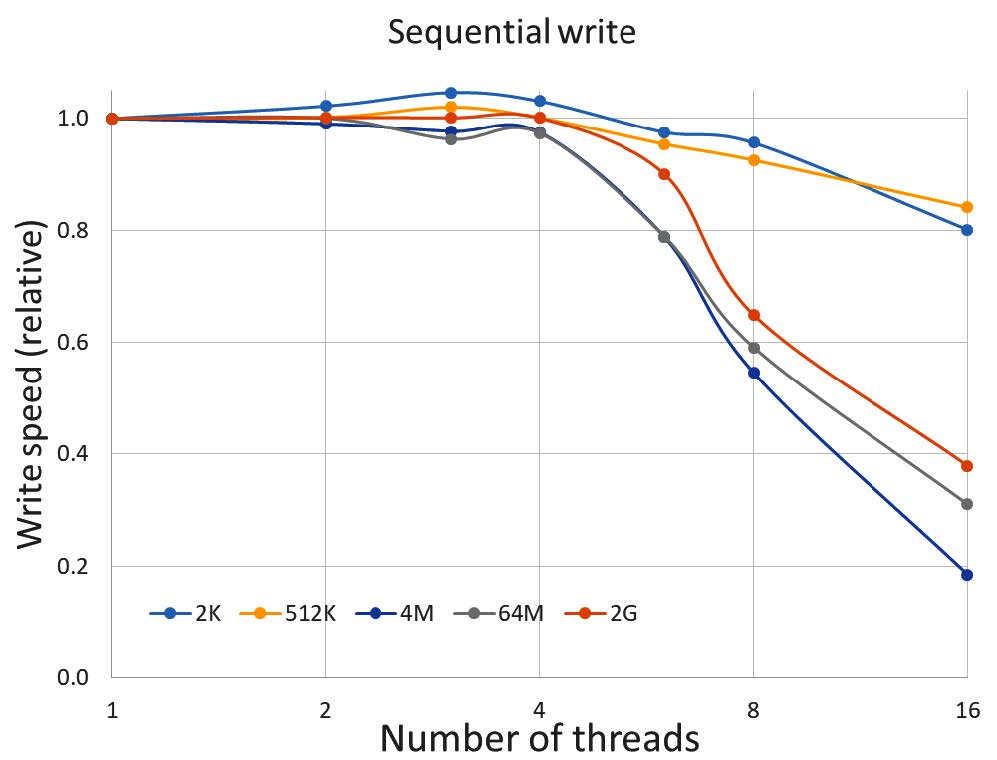
\includegraphics[width=0.7\textwidth]{content/1/chapter5/images/3.jpg}\\
图5.3 - 内存吞吐量(相对于单个线程的吞吐量),以及线程数量
\end{center}

随着内存速度的标准化,所以单线程总是1,对于适合L1或L2缓存的小数据集,每个线程的内存速度几乎保持不变,即使是16个线程(每个线程的写入速度是单线程速度的80\%)。然而,当进入L3缓存或超过它的大小,4个线程之后速度就会下降。从8个线程增加到16个线程性能改进就非常小了。系统中没有足够的带宽以足够快的速度将数据写入内存。

尽管用于读取内存的带宽通常比用于写入的带宽稍好一些,但不同内存访问模式的结果看起来非常接近。

可以看到,如果程序在单线程的情况下内存受限,那么性能就会受到在主内存中移动数据速度的限制。我们可以期望从并发性中获得的性能改进时,就要受到相当严格的限制。若这不适用于你,可能是因为你没有一个16核处理器,便宜的处理器有便宜的内存总线,所以大多数4核系统也没有足够的内存带宽给所有的核。

对于多线程程序,更重要的是要避免内存限制。这里使用的技术是分割计算,这样可以在更小的数据集上完成更多的工作,这些数据集适合存放于L1或L2缓存,再重新安排计算,这样可以用更少的内存访问完成更多的工作,通常会以重复一些计算为代价。优化内存访问模式,这样内存是顺序访问,而不是随机访问(即使可以饱和这两种访问模式,顺序访问的总带宽要大得多,因此对于相同数量的数据,如果使用随机访问,程序可能会受到内存限制,而如果使用顺序访问,则完全不受内存速度的限制)。仅靠实现技术是不够的,并且不能产生预期的性能改进,那么下一步就是使算法适应并发编程的实际情况:许多问题都有多个算法,它们的内存需求不同。对于单线程程序来说,最快的算法通常会被另一种更适合并发的算法所超越:我们在单线程执行速度上的损失,可以通过可扩展执行来弥补。

目前为止,我们假设每个线程都独立于所有其他线程完成自己的工作。由于对有限资源(如内存带宽)的争用,线程之间的惟一交互是间接的。这是最容易编写的程序,但大多数实际情况中的程序不允许这样的限制。这带来了一系列全新的性能问题,是时候来了解这些问题了。


















